
\section{Introduction}

\begin{figure}[t]
  \includegraphics[width=\columnwidth]{fig/RUMAD_comparison.pdf}
  \caption{\newtext{Comparison of accuracy and average token cost. 
  Accuracy for MMLU ($\bullet$) and GSM8K ($\blacksquare$) corresponds to the left Y-axis, while GPQA (\textbf{$\blacktriangle$}) corresponds to the right Y-axis. 
  Points closer to the top-left corner represent a superior accuracy-efficiency trade-off. 
  The results show that RUMAD variants consistently outperform baselines by achieving higher accuracy at a lower token cost.}}
  \label{fig:RUMAD_comparison}
  \Description{Comparison of accuracy and token consumption. The results show that RUMAD achieves better trade-off between accuracy and efficiency.}
\end{figure}

\begin{table*}[t]
\centering
\caption{Different types of MAD methods are designed from different strategies. Mark $\bullet$ indicates corresponding metrics are taken into design target. Mark $\circ$ indicates methods may have side-effect on corresponding metrics but don't focus on them. Mark - means methods fail on corresponding aspects.}
\begin{tabular}{lccc}
\toprule
                            & Static Topology Methods & External-LLM Methods & \textbf{RUMAD}  \\ \midrule
Accuracy                    & $\bullet$                  & $\bullet$               & $\bullet$ \\
Consensus                   & $\circ$                    & $\bullet$               & $\bullet$ \\
External Opinion Independent & $\bullet$                  & -                    & $\bullet$ \\
Question Independent        & $\bullet$                  & -                    & $\bullet$ \\
Communication Cost Control  & $\circ$                    & $\circ$                 & $\bullet$ \\ \bottomrule
\end{tabular}
\label{tab:Methods_list}
\end{table*}

Multi-agent debate (MAD) frameworks harness the collective intelligence of multiple large language models (LLMs) \citep{touvron2023llama,zhao2023survey, naveed2023comprehensive,jiang2024survey,achiam2023gpt,glm2024chatglm,guo2025deepseek} to achieve superior reasoning and decision-making beyond what any single model can attain. However, the effectiveness and practicality of MAD systems fundamentally depend on how agents communicate and exchange information during debate \citep{liang2023encouraging}.

\newtext{\textbf{Adaptivity}:} Most existing MAD approaches utilize static sparse topologies, such as Sparse MAD (S-MAD) \citep{li2024improving}, Group Debate (GD) \citep{liu2024groupdebate} or Selective Sparse MAD (S$^2$-MAD) \citep{zeng2025s} using ring, star, or fixed grouped/hierarchical structures, to reduce the communication burden compared to fully connected networks \citep{du2023improving,hill2015real,sun2023corex}. Such methods  inherently lack flexibility. \newtext{Fixed topologies cannot adapt to the evolving diversity, difficulty, or semantic style changes present across different tasks (e.g., allocating the same budget to an easy and a hard problem).} As a result, they easily either cut off valuable information paths for complex tasks or retain redundant, low-value connections on simple tasks, ultimately hampering both efficiency and collective reasoning. 

\newtext{\textbf{Privacy}: Some adaptive methods introduce external LLM-based “judger” or “summarizer” roles, where a larger often more powerful agent (e.g GPT-4) supervises the debate. 
% However, such schemes may lead to \textit{capability intrusion}. 
Context within a debate is exposed to external models. External knowledge in return suppresses the diversity and emergent collaboration of internal agent swarm.}

\newtext{\textbf{Efficiency}:}A further critical limitation of existing MAD approaches is the lack of explicit modeling of token cost. Most previous MAD designs focus solely on accuracy or consensus, overlooking the real-world computational and financial constraints imposed by large-scale LLM deployments. Without a principled framework for managing communication budgets, these systems either waste excessive resources or struggle to generalize under practical constraints. Static methods typically impose a hard upper bound on communication rounds by restricting the debate topology. 
% This type of design is based more on some empirical rules or artificial rules rather than systematic and theoretical considerations of resource allocation. 
% In contrast, approaches that incorporate external LLMs as judges or coordinators can, in principle, leverage the LLM’s reasoning ability to perform some form of budget control. However, this effect is more of a open-loop byproduct rather than a principled mechanism—budgeting emerges implicitly through prompting and remains inherently uncontrollable and unpredictable, as it depends entirely on the LLM’s internal judgment rather than transparent or tunable criteria.

Major challenges arise in balancing accuracy, diversity and efficiency(communication budget) of MAD, as show in Table~\ref{tab:Methods_list}. \newtext{To address these challenges, we propose \textbf{RUMAD} (\textbf{\textit{Reinforcement-Unifying Multi-Agent Debate}}), a novel framework that formulates dynamic agent coordination and topology control as a reinforcement learning (RL) problem, without external LLM utilization.} 

RUMAD formulates dynamic communication topology control as a reinforcement learning (RL) problem that is fundamentally independent of debate content. Specifically, we represent the communication topologies among agents as a dynamic weighted directed graph, where a non-LLM RL agent dynamically adjusts the edge weights in response to the evolving debate context. \newtext{Crucially, the RL controller is \textbf{content-agnostic}}: it does not intervene in the reasoning process or rely on privileged knowledge, but instead observes \newtext{\textbf{high-level structural dynamics}} such as semantic similarity \newtext{scalars}, answer agreement, debate progress, and communication cost. By modeling observations in this manner, RUMAD preserves the neutrality of dynamic debate management and effectively mitigates the risk of introducing external opinions or privileged information into the reasoning process. 

RUMAD constructs a multi-objective reward function that explicitly balances accuracy, consensus, and token efficiency, while strictly enforcing communication budget constraints. We employ the PPO algorithm to train the topology control agent, which can achieve these trade-offs after only lightweight training. More importantly, the content-agnostic and neutral design of RUMAD endows it with strong zero-shot generalization capability, enabling robust performance across diverse tasks and domains without the need for task-specific finetuning.

Our experiments on standard benchmarks, including \textbf{MMLU} \citep{hendrycks2020measuring}, \textbf{GSM8K} \citep{cobbe2021training}, and \textbf{GPQA} \citep{reinGPQAGraduateLevelGoogleProof2023}, demonstrate that RUMAD achieves a superior balance between collective accuracy and token usage compared to both fully-connected and static sparse baselines. \newtext{As shown in Figure~\ref{fig:RUMAD_comparison}, take GSM8K for example, RUMAD$_{B=12}$ requires only 0.121k tokens per percentage point of accuracy, and RUMAD$_{B=18}$ requires 0.195k, compared to the 0.354k tokens required by the second-best baseline (GD).} Concretely, RUMAD reduces token cost by 80\% while improving accuracy on MMLU, and robustly generalizes to new tasks (GPQA, GSM8K) with similar performance.

\textbf{Our contributions are summarized as follows:}

\begin{itemize}
    \item We propose RUMAD, a novel reinforcement learning framework that dynamically controls multi-agent debate topologies to optimize both accuracy and efficiency.
    \item We design a unified, content-agnostic observation and reward scheme that enables robust and generalizable learning of communication strategies across tasks and agent configurations.
    \item We empirically demonstrate that RUMAD outperforms both fully connected and static sparse MAD baselines, achieving superior trade-offs between performance and cost on multiple challenging benchmarks.
\end{itemize}


\begin{figure*}[t]
  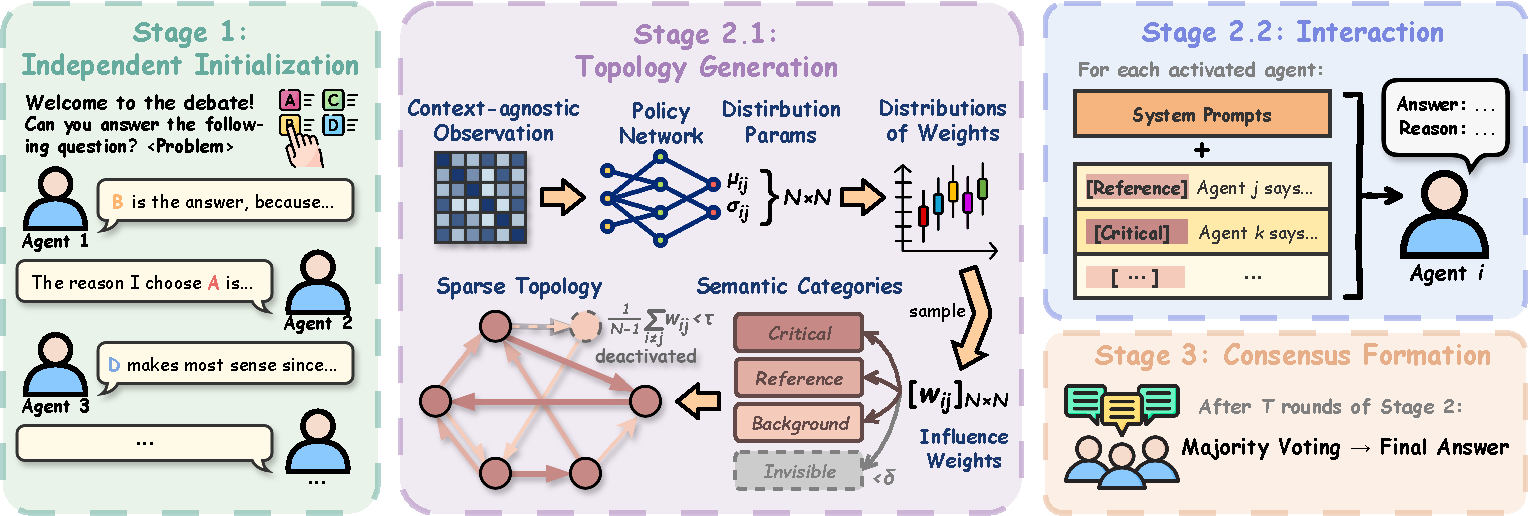
\includegraphics[width=\textwidth]{fig/RUMAD_pipeline.pdf}
  \caption{The process pipeline of RUMAD. In the first stage, all agents gives the initial response. In the second stage, RUMAD organizes topology in stage 2.1 and the selected agents debate with each other in stage 2.2. In the last stage, the final decision is obtained via majority voting.}
  \Description{The process pipeline of RUMAD. In the first stage, all agents gives the initial response. In the second stage, RUMAD organizes topology in stage 2.1 and the selected agents debate with each other in stage 2.2. In the last stage, the final decision is obtained via majority voting.} 
  \label{fig:process_pipeline}
\end{figure*}
